\section{Data generation for the sphere}\label{sec:data_generation_sphere}
A significant challenge in this project has been obtaining high-quality data for training data-driven methods on a sphere.
To tackle this, we are exploring various approaches for data generation, including the potential to create our own data and utilize external data sources.


\subsection*{Projecting 2D data to the sphere}
Our initial approach involved projecting the solution data from the 2D SWE onto the sphere.
To ensure stability and generate high-quality data, we set the CFL number to 0.8.
The coordinates $\theta$ (longitude) and $\phi$ (latitude) are treated similarly to $x$ and $y$ in the 2D case.
The grid is configured with $N_{\theta} = 200$ grid points in the $\theta-$direction and $N_{\phi} = 100$ grid points in the $\phi-$direction.
The higher resolution in the $\theta-$direction accounts for its double distance compared to the $\phi-$direction.
We use a Gaussian function as initial condition
\begin{align*}
    h(\theta, \phi, 0) = h_0 + a \cdot \exp\left( -\frac{{(\theta - \theta_c)}^2 + {(\phi - \phi_c)}^2}{{(2\sigma)}^2} \right),
\end{align*}
where $h_0 = 1$ m, $a = 3$, $\theta_c = \frac{3 \pi}{2}, \phi_c = \frac{\pi}{3}$, and $\sigma = \frac{\pi}{16}$.
The SWE are solved from $t = 0$ s to $t_{\text{end}} = 0.5$ s, using a variable step size $\Delta t$.
The simulation takes 199 time steps, resulting in an average time step size of $\Delta t \approx 0.0025$ s.
This value is significantly smaller than in the 2D case, likely due to the higher number of grid points, another domain and lower CFL number.
The results after some given time steps are presented in~\autoref{fig:sphere_projected_water_height_timesteps}.
\begin{figure}[H]
    \centering
    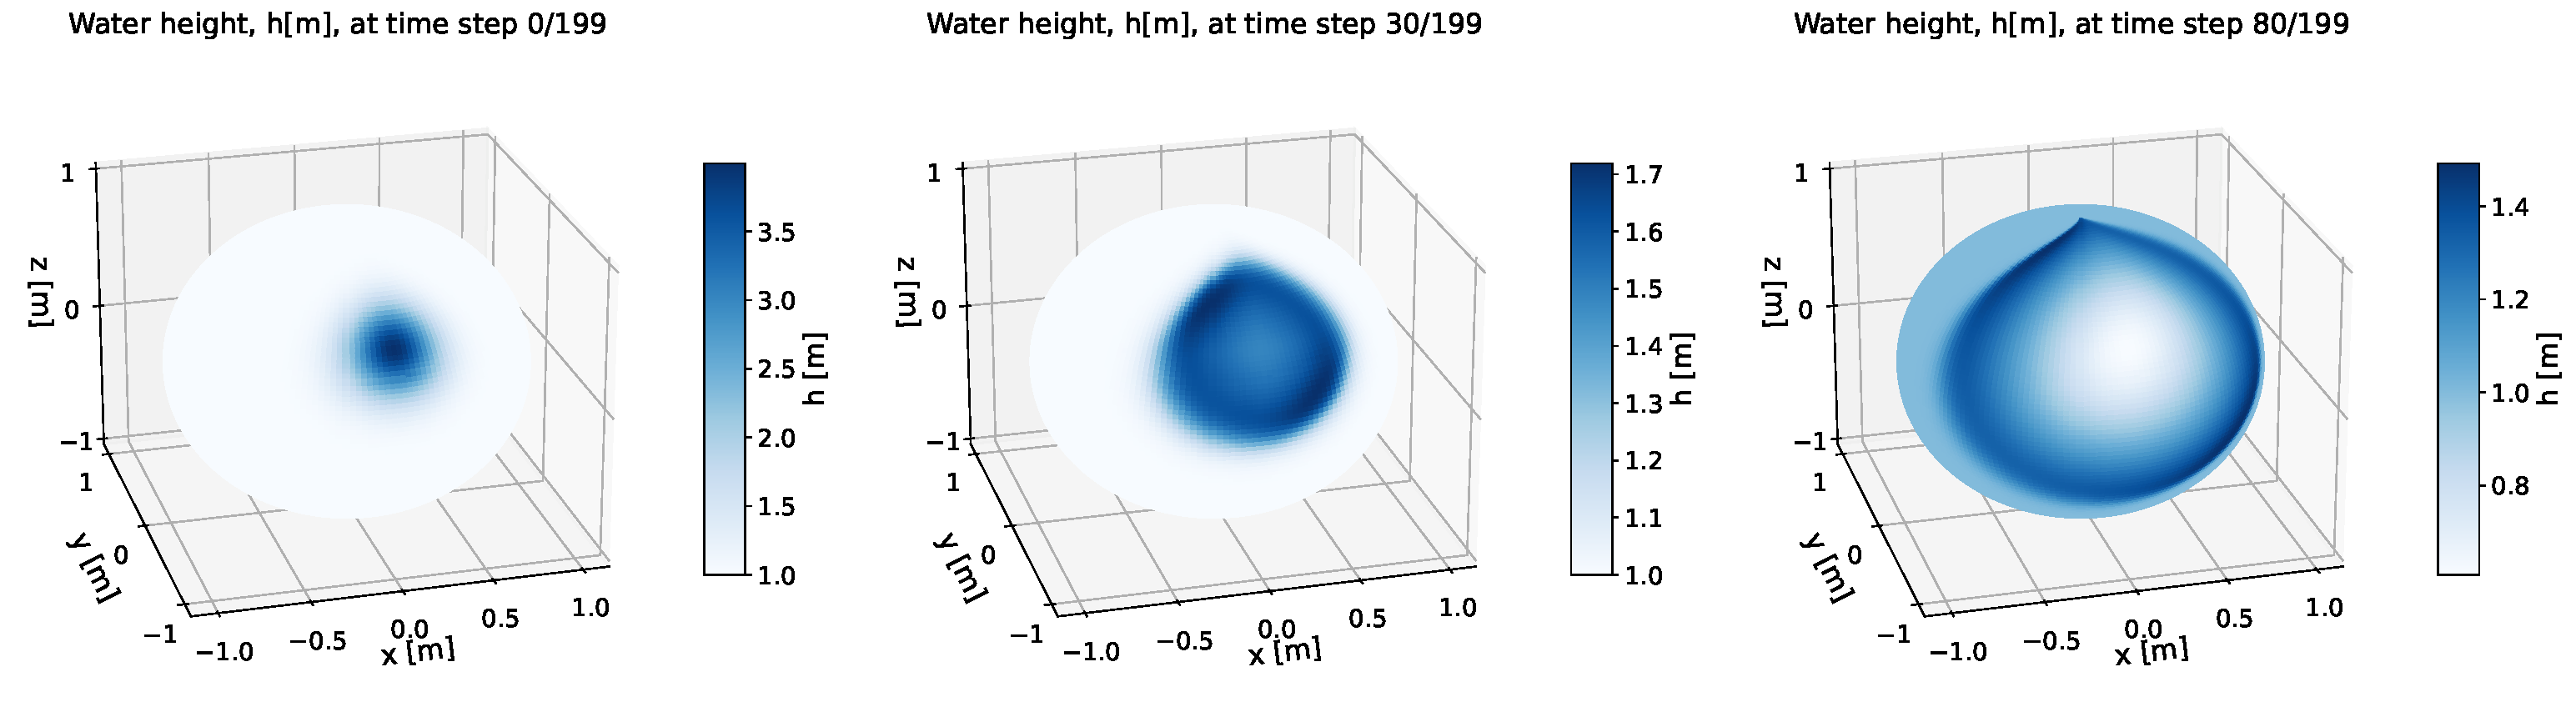
\includegraphics[width=0.95\textwidth]{C:/Users/Matteo/Shallow-Water-Equations/plots/sphere_projected_water_height_timesteps.pdf}
    \caption{Water height on the sphere for different timesteps.}\label{fig:sphere_projected_water_height_timesteps}
\end{figure}
In~\autoref{fig:sphere_projected_water_height_timesteps} we observe the evolution of the water height over time on the sphere.
The initial Gaussian bump propagates across the sphere, but singularities are present, especially at the poles.
These issues arise, among other things, from neglecting the curvature of the sphere. 
While this approach might be acceptable for some applications, for instance when focusing on a small region near the equator, where the projection is more accurate, it is not suitable for our project.
Since our aim is to model the entire sphere, accounting for its curvature is essential.
Consequently, we cannot use this data.

\subsection*{Mesh generation for the sphere}
To solve the SWE on the sphere, we must use a different grid than the regular grid used in the 2D case.
One approach is to use an icosahedral grid, which approximates the sphere with triangles.
The grid structure allows for various levels of refinement, depending on the desired level of accuracy.
At each refinement level, the number of triangles increases by a factor of four, as each triangle is divided into four smaller triangles, meaning that the number of triangles increases drastically with each level of refinement.
The grid is generated using Matlab code from the Github repository~\cite{sphere_mesh_triangles} and then rewritten to Python.
The first four levels of refinement are shown in~\autoref{fig:icosahedral_grid}.
\begin{figure}[H]
    \centering
    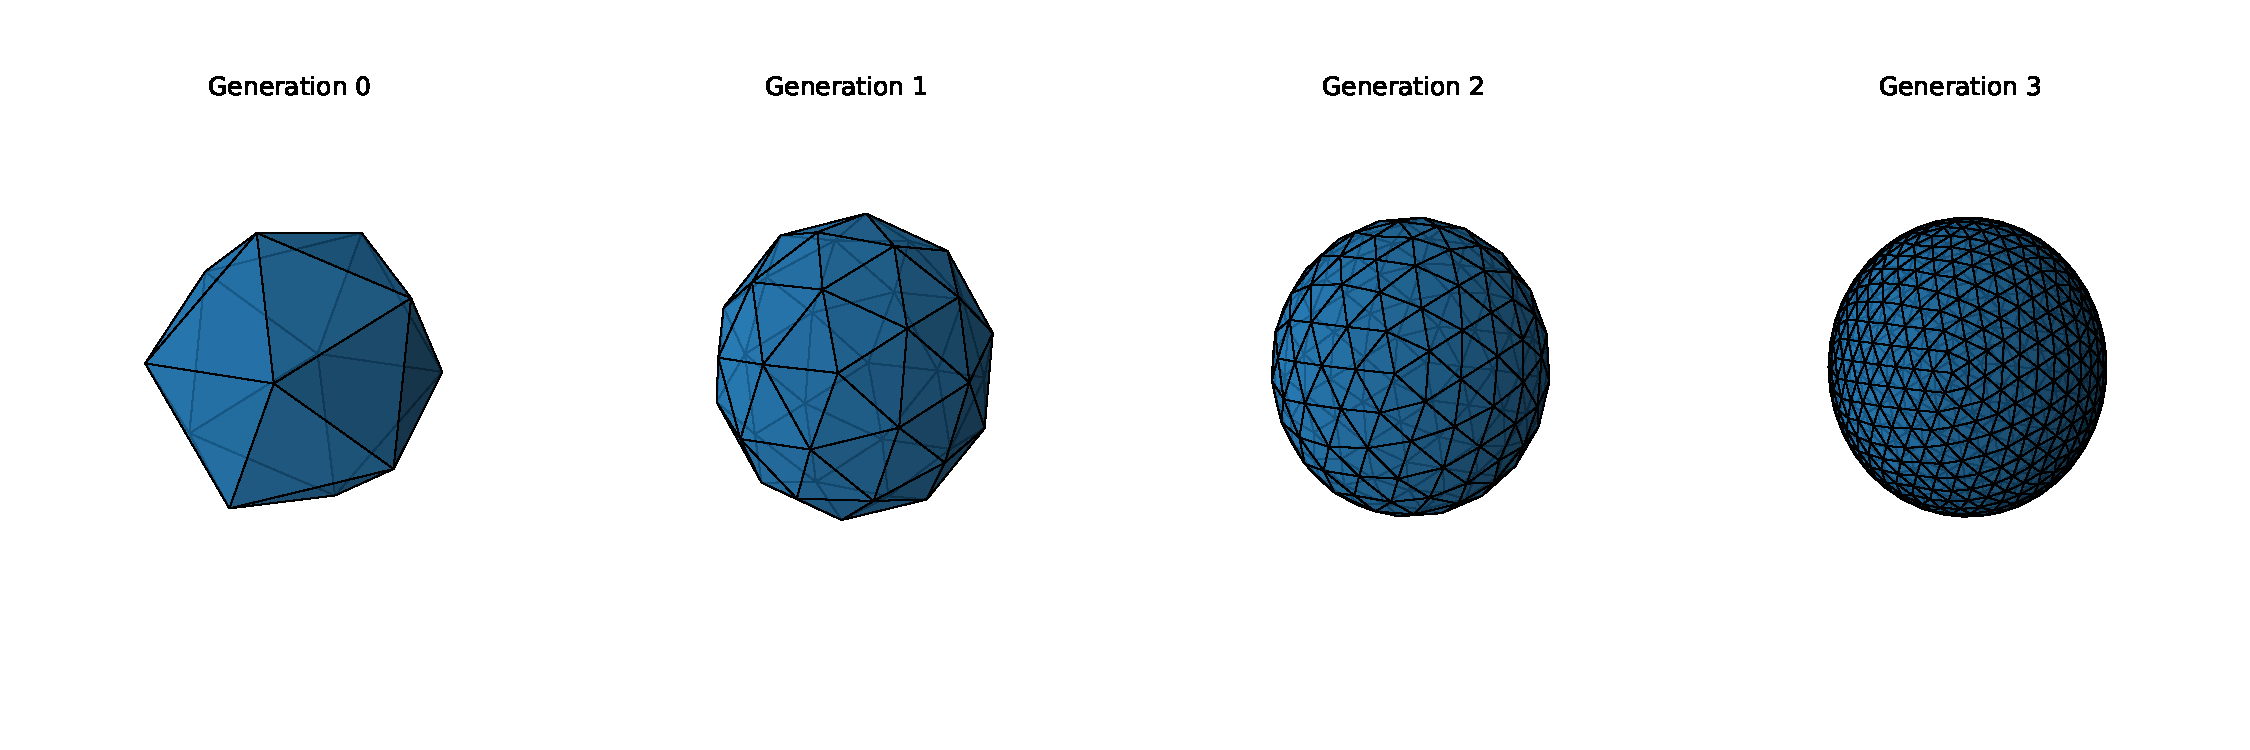
\includegraphics[width=\textwidth]{C:/Users/Matteo/Shallow-Water-Equations/plots/icosahedral_mesh_refinement.pdf}
    \caption{Icosahedral grid for the first 4 levels of refinement.}\label{fig:icosahedral_grid}
\end{figure}
In~\autoref{fig:icosahedral_grid} we see how the grid is refined at each level, resulting in a progressively more accurate representation of the sphere.
We will brieftly outline the process of solving the SWE on this grid structure, inspired by the finite element method (FEM).
The main idea is to keep track of which neighboring triangles each triangle has, as well as which interfaces they share.
Each triangle is numbered, as well as each vertex.
This information is organized into three key tables:
\begin{itemize}
    \item Element-to-Vertex (EToV) table. This table stores the vertices of each triangle.
    Each row corresponds to a triangle, and the three columns correspond to the three vertices of the triangle.
    \item Element-to-Element (EToE) table. Derived from the EToV table, this table stores the neighboring triangles of each triangle.
    Each row corresponds to a triangle, and the three columns correspond to the three neighboring triangles. 
    \item Element-to-Face (EToF) table. Keeps track of which faces (edges) are shared between two triangles.
    Each row corresponds to a triangle, and the columns correspond to the neighboring triangles and the face they share.
\end{itemize}
The method involves computing fluxes across interfaces between triangles.
For each interface, the flux leaving one triangle and entering its neighbor is calculated to ensure the total flux across the system is zero, conserving the total volume of water.
However, since the triangles are not aligned in straight lines, as in the 2D case, we must consider the contributions in both the $\theta-$ and $\phi-$directions for each interface flux.
Previously, we could view the problem as two 1D problems, but now they are intertwined, highlighting the complexity of the problem.

\subsection*{External data sources}
Another approach for obtaining data is to use external data sources.
One possible source is the Copernicus climate data store, specifically the ORAS5 global ocean reanalysis dataset, which provides monthly data from 1958 to the present~\cite{Copernicus_data}.
For this study, we focus on the sear surface height, defined as the vertical distance between the actual sea surface and a reference surface, representing a mean sea level if the ocean were at rest.
The data is a 2D field, depending on the longitude and latitude.
To get an overview of the data, we downloaded the data from January to December 2014 and plotted the sea surface height as the difference from the reference sea surface height.
The plots for January to April are shown in~\autoref{fig:copernices-ssh}.
\begin{figure}[H]
    \centering
    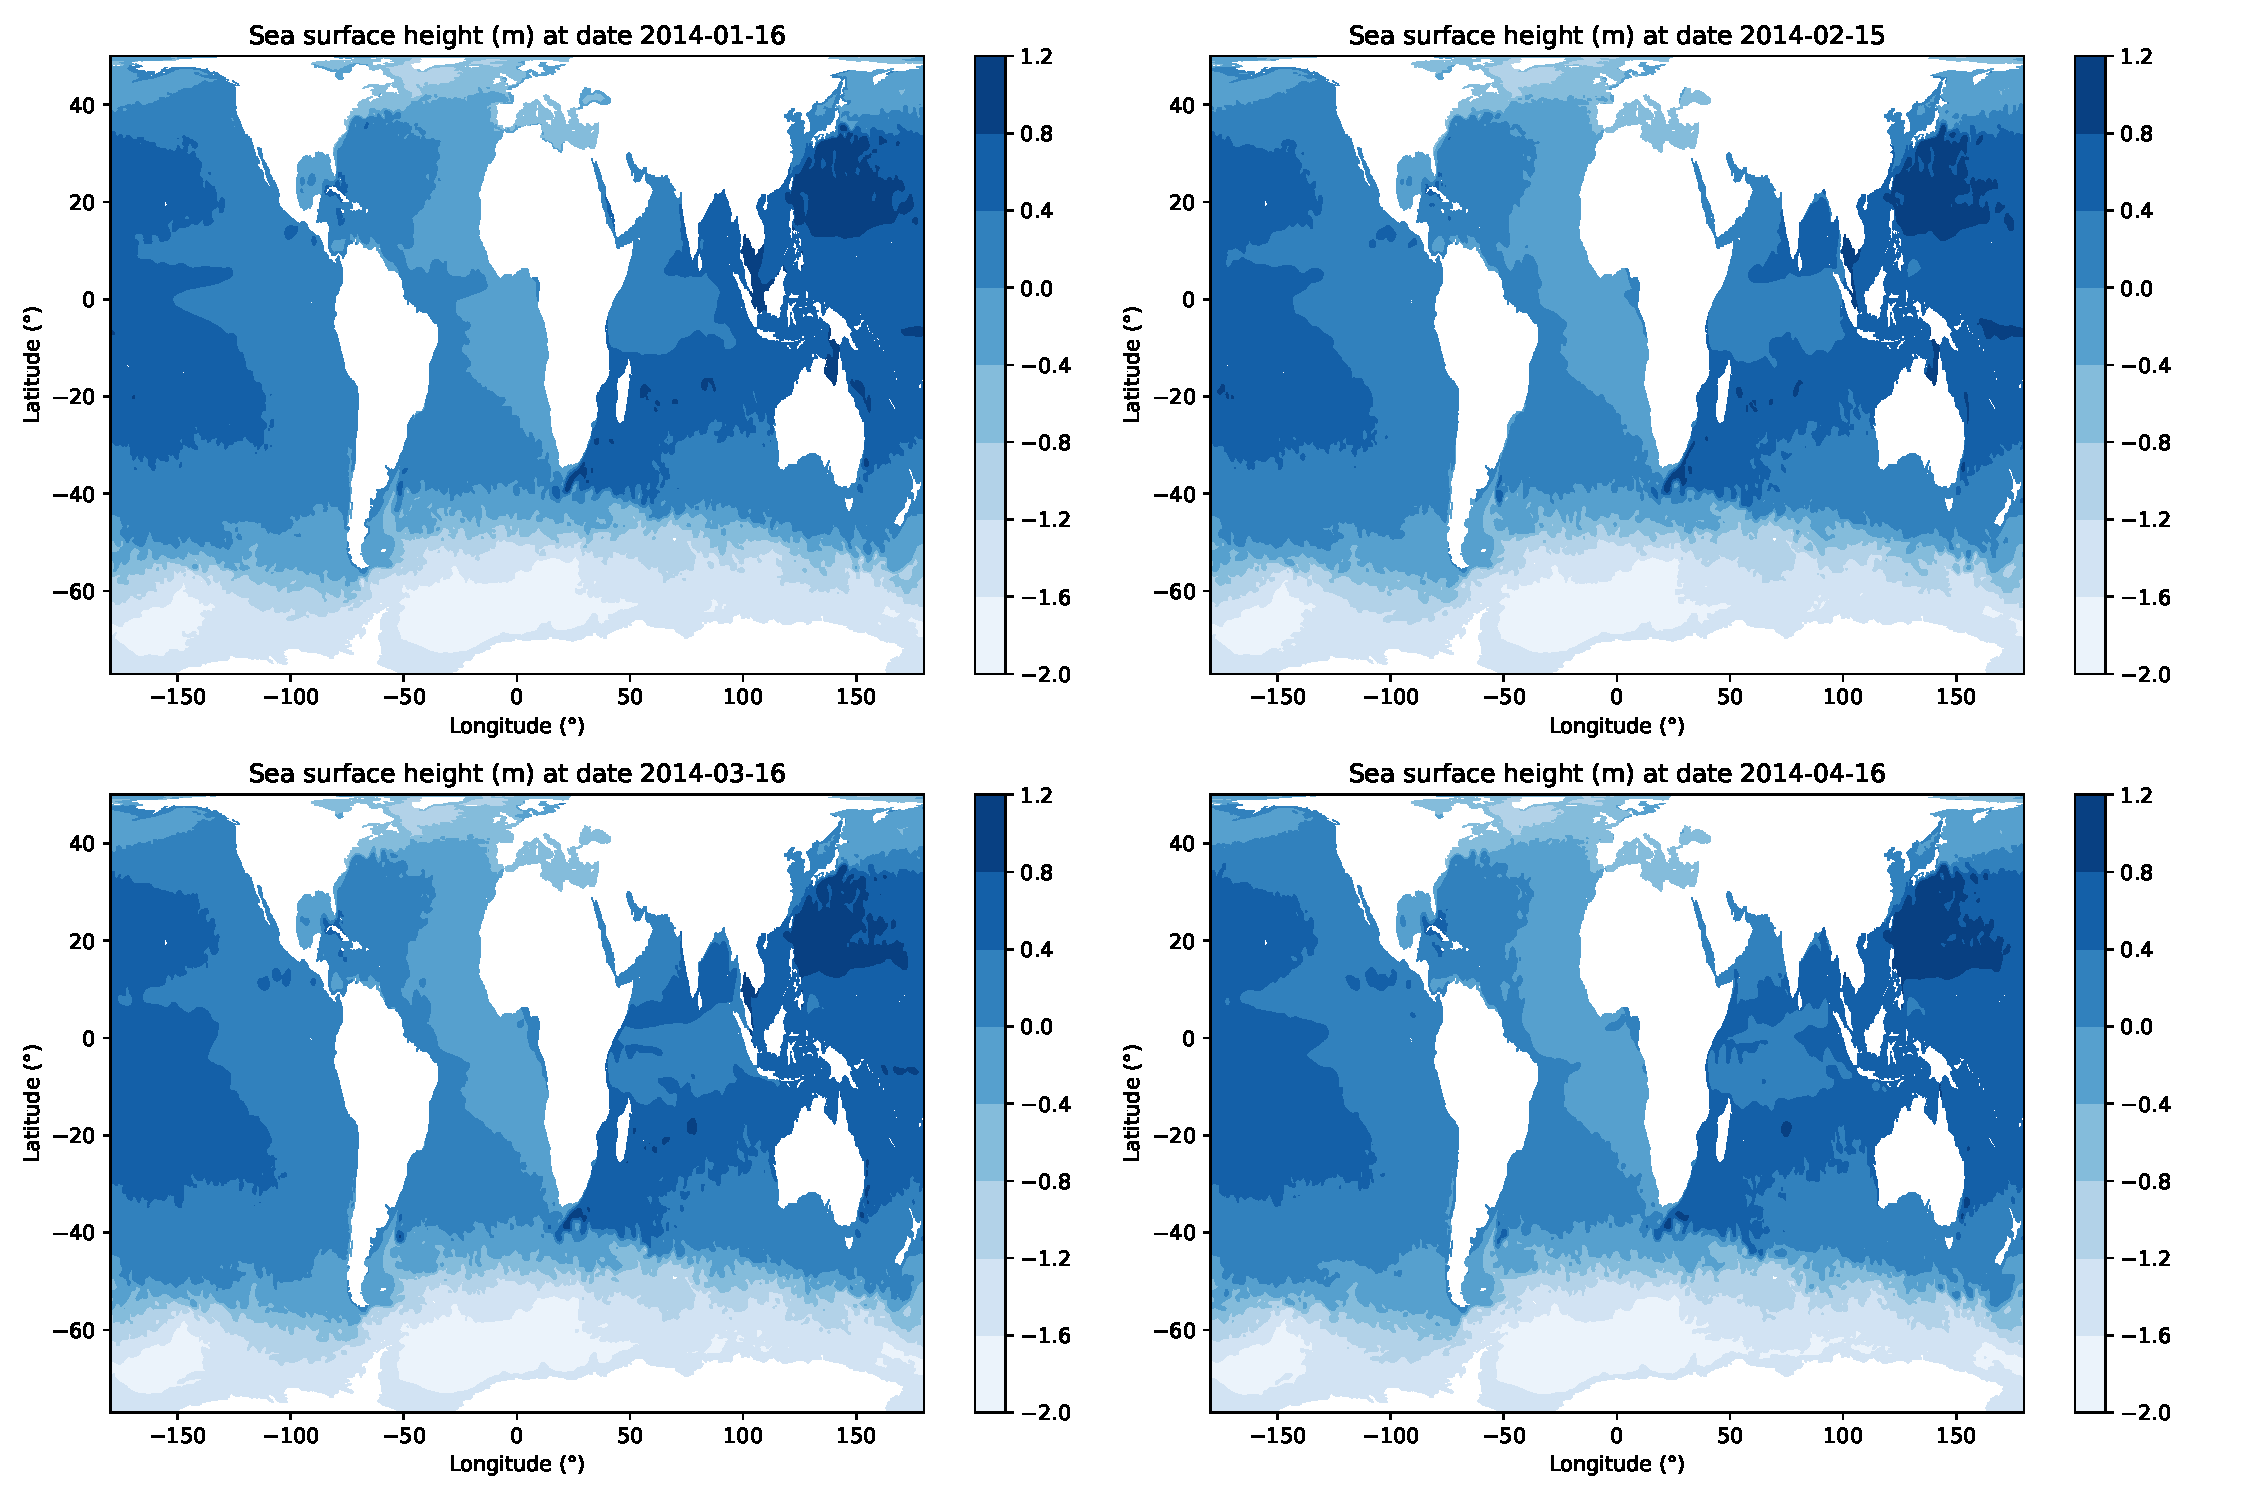
\includegraphics[width=0.95\textwidth]{C:/Users/Matteo/Shallow-Water-Equations/plots/ssh_field.pdf}
    \caption{Sea surface height as the diffference from reference sea surface height for the months Jan-Apr 2014.}\label{fig:copernices-ssh}
\end{figure}
Note that the data was recently updated (2025-01-15).
At the time of downloading, we obtained the newest data available.
While training an SFNO on real-world data could be an exciting prospect, we have decided not to proceed with this data set due to several uncertainties.
In particular, since we cannot fully account for the quality and reliability of the data, we have chosen not to pursue this approach.

